\title{EE5311 -- Assignment 6}
\author{Joyen Benitto}
\date{\today}
\maketitle

\section{Circuit}

\subsubsection{Schematic}

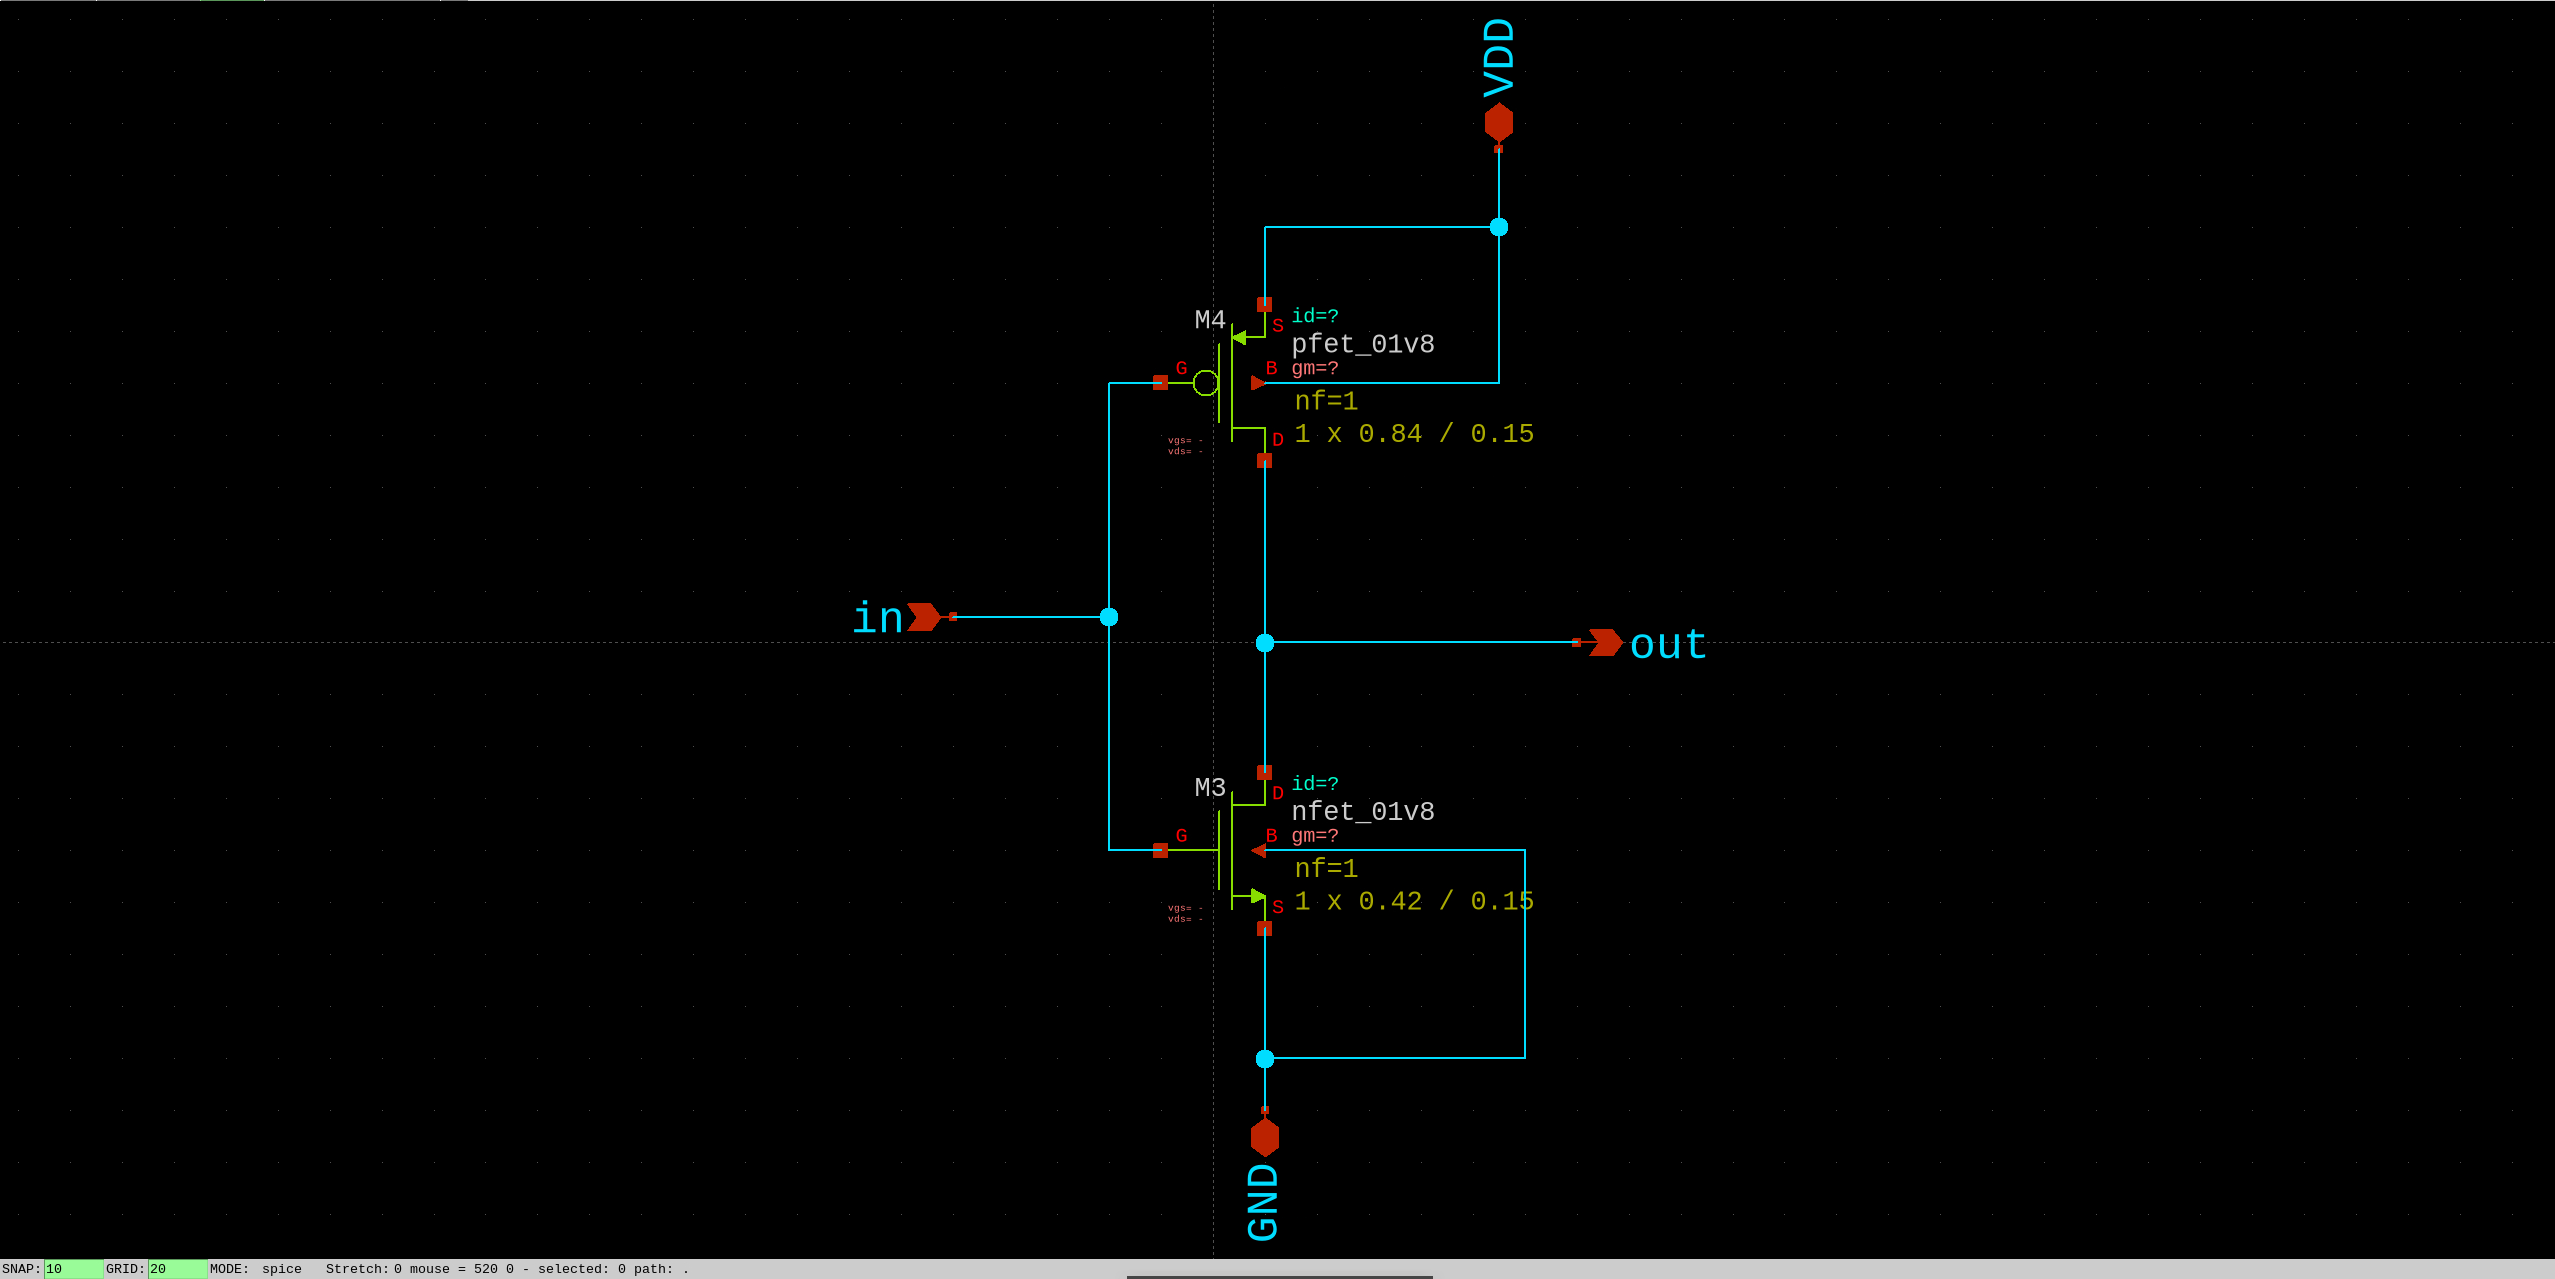
\includegraphics[width=0.75\textwidth]{figures/inv_schematic.png}

\textbf{Figure 1:} \texttt{inv.sch} -- static CMOS inverter, $1\times0.84/0.15$
pMOS, $1\times0.42/0.15$ nMOS

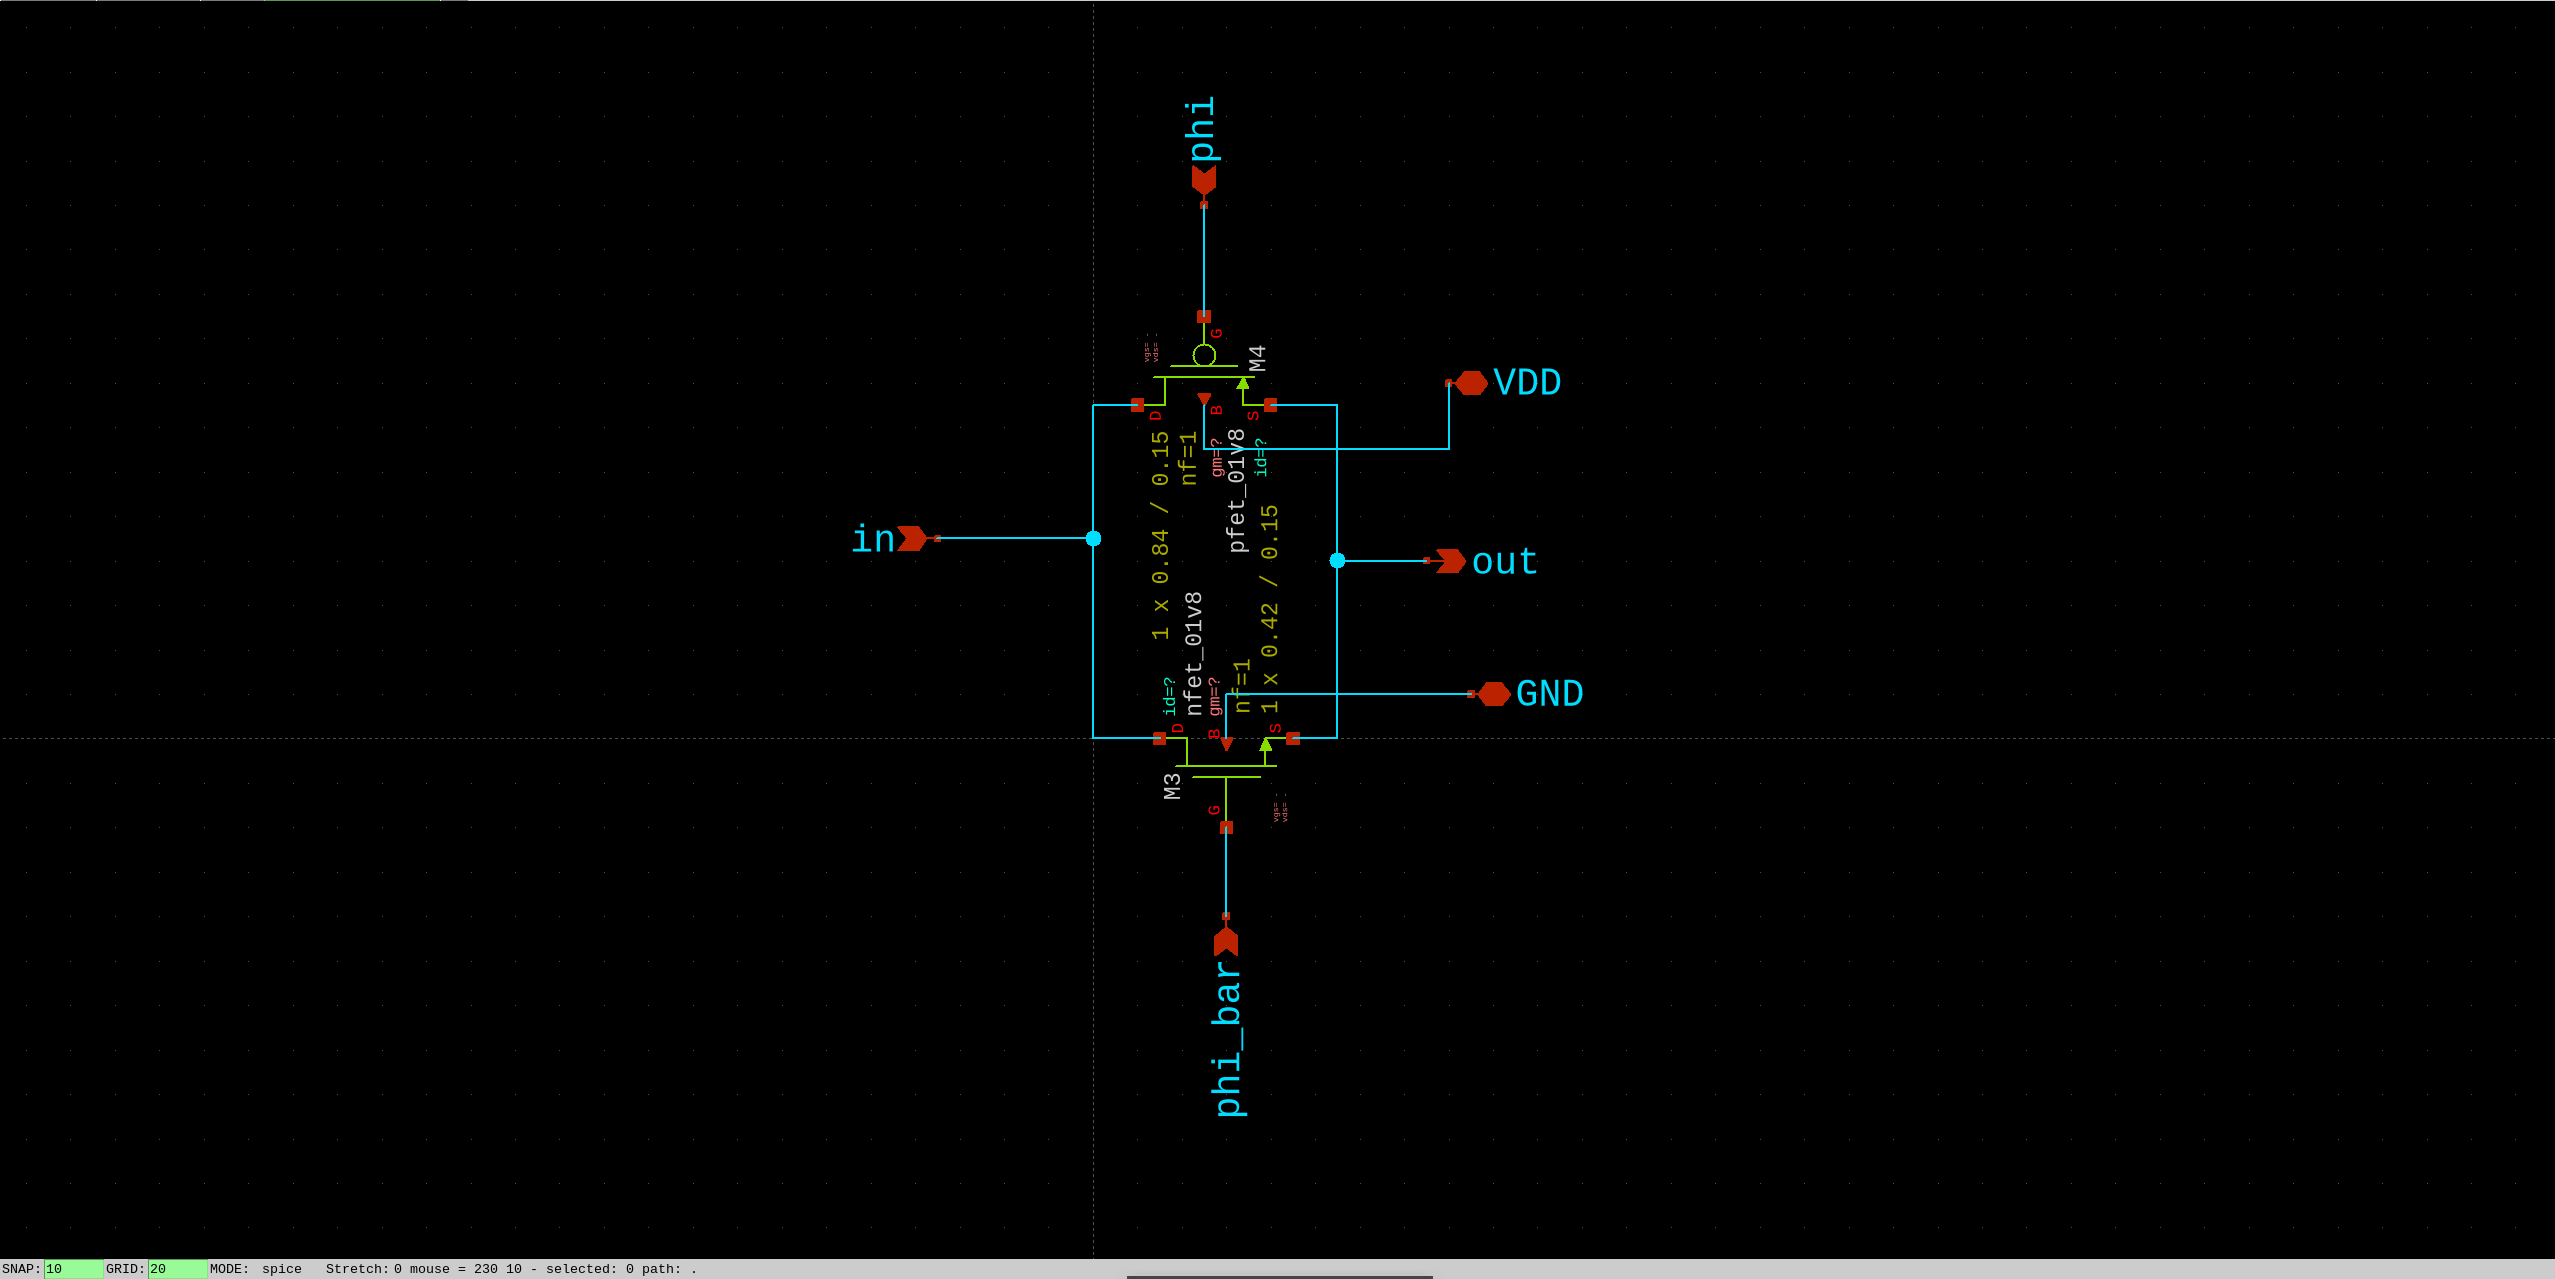
\includegraphics[width=0.75\textwidth]{figures/transmission_gate_schematic.png}

\textbf{Figure 2:} \texttt{transmission\_gate.sch} -- CMOS transmission gate,
same device sizes, gated by \texttt{phi} / \texttt{phi\_bar}

%%------------------------------------------------------------------------------
\section{Problem 1(a): rising edge}

\subsubsection{Schematic}

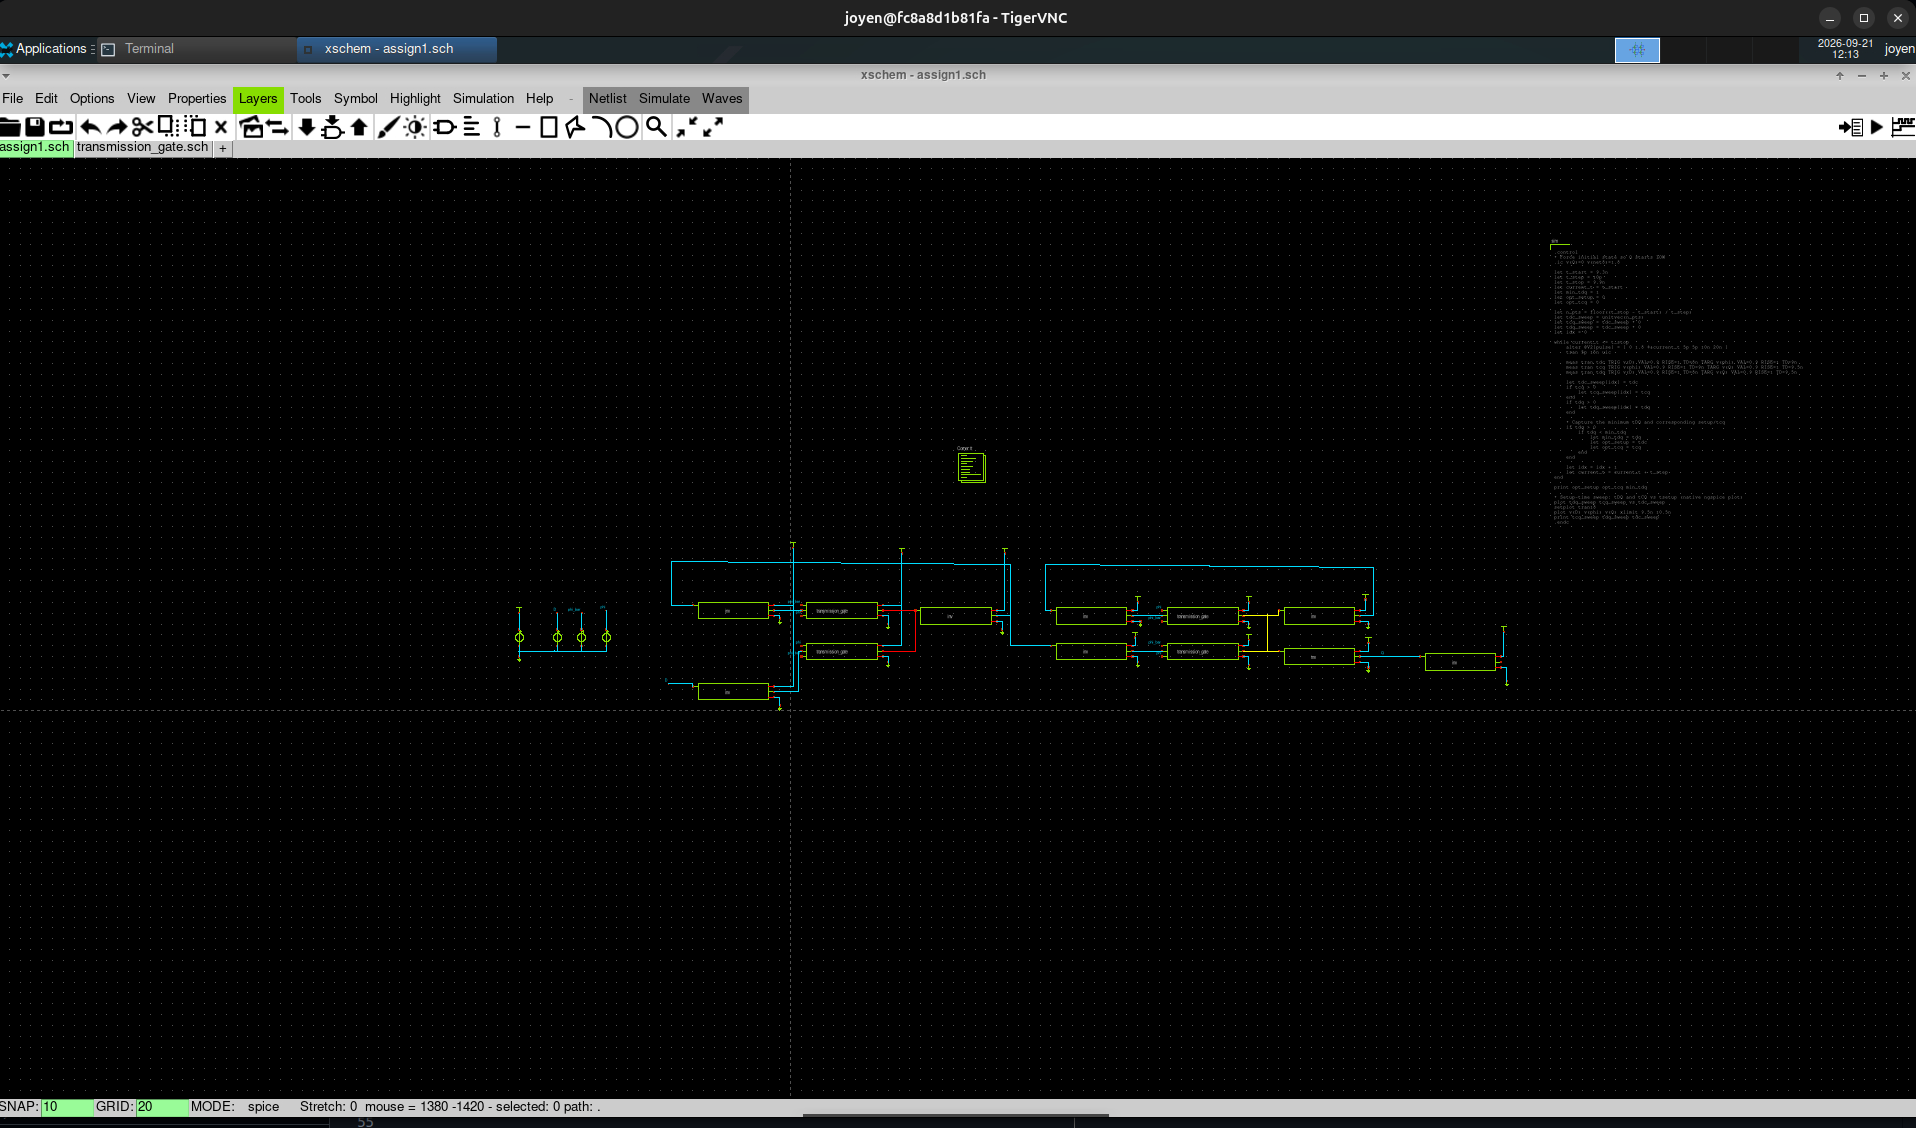
\includegraphics[width=0.95\textwidth]{figures/assign1_schem.png}

\textbf{Figure 3:} \texttt{assign1.sch} -- flip-flop testbench

\subsubsection{Measurement}

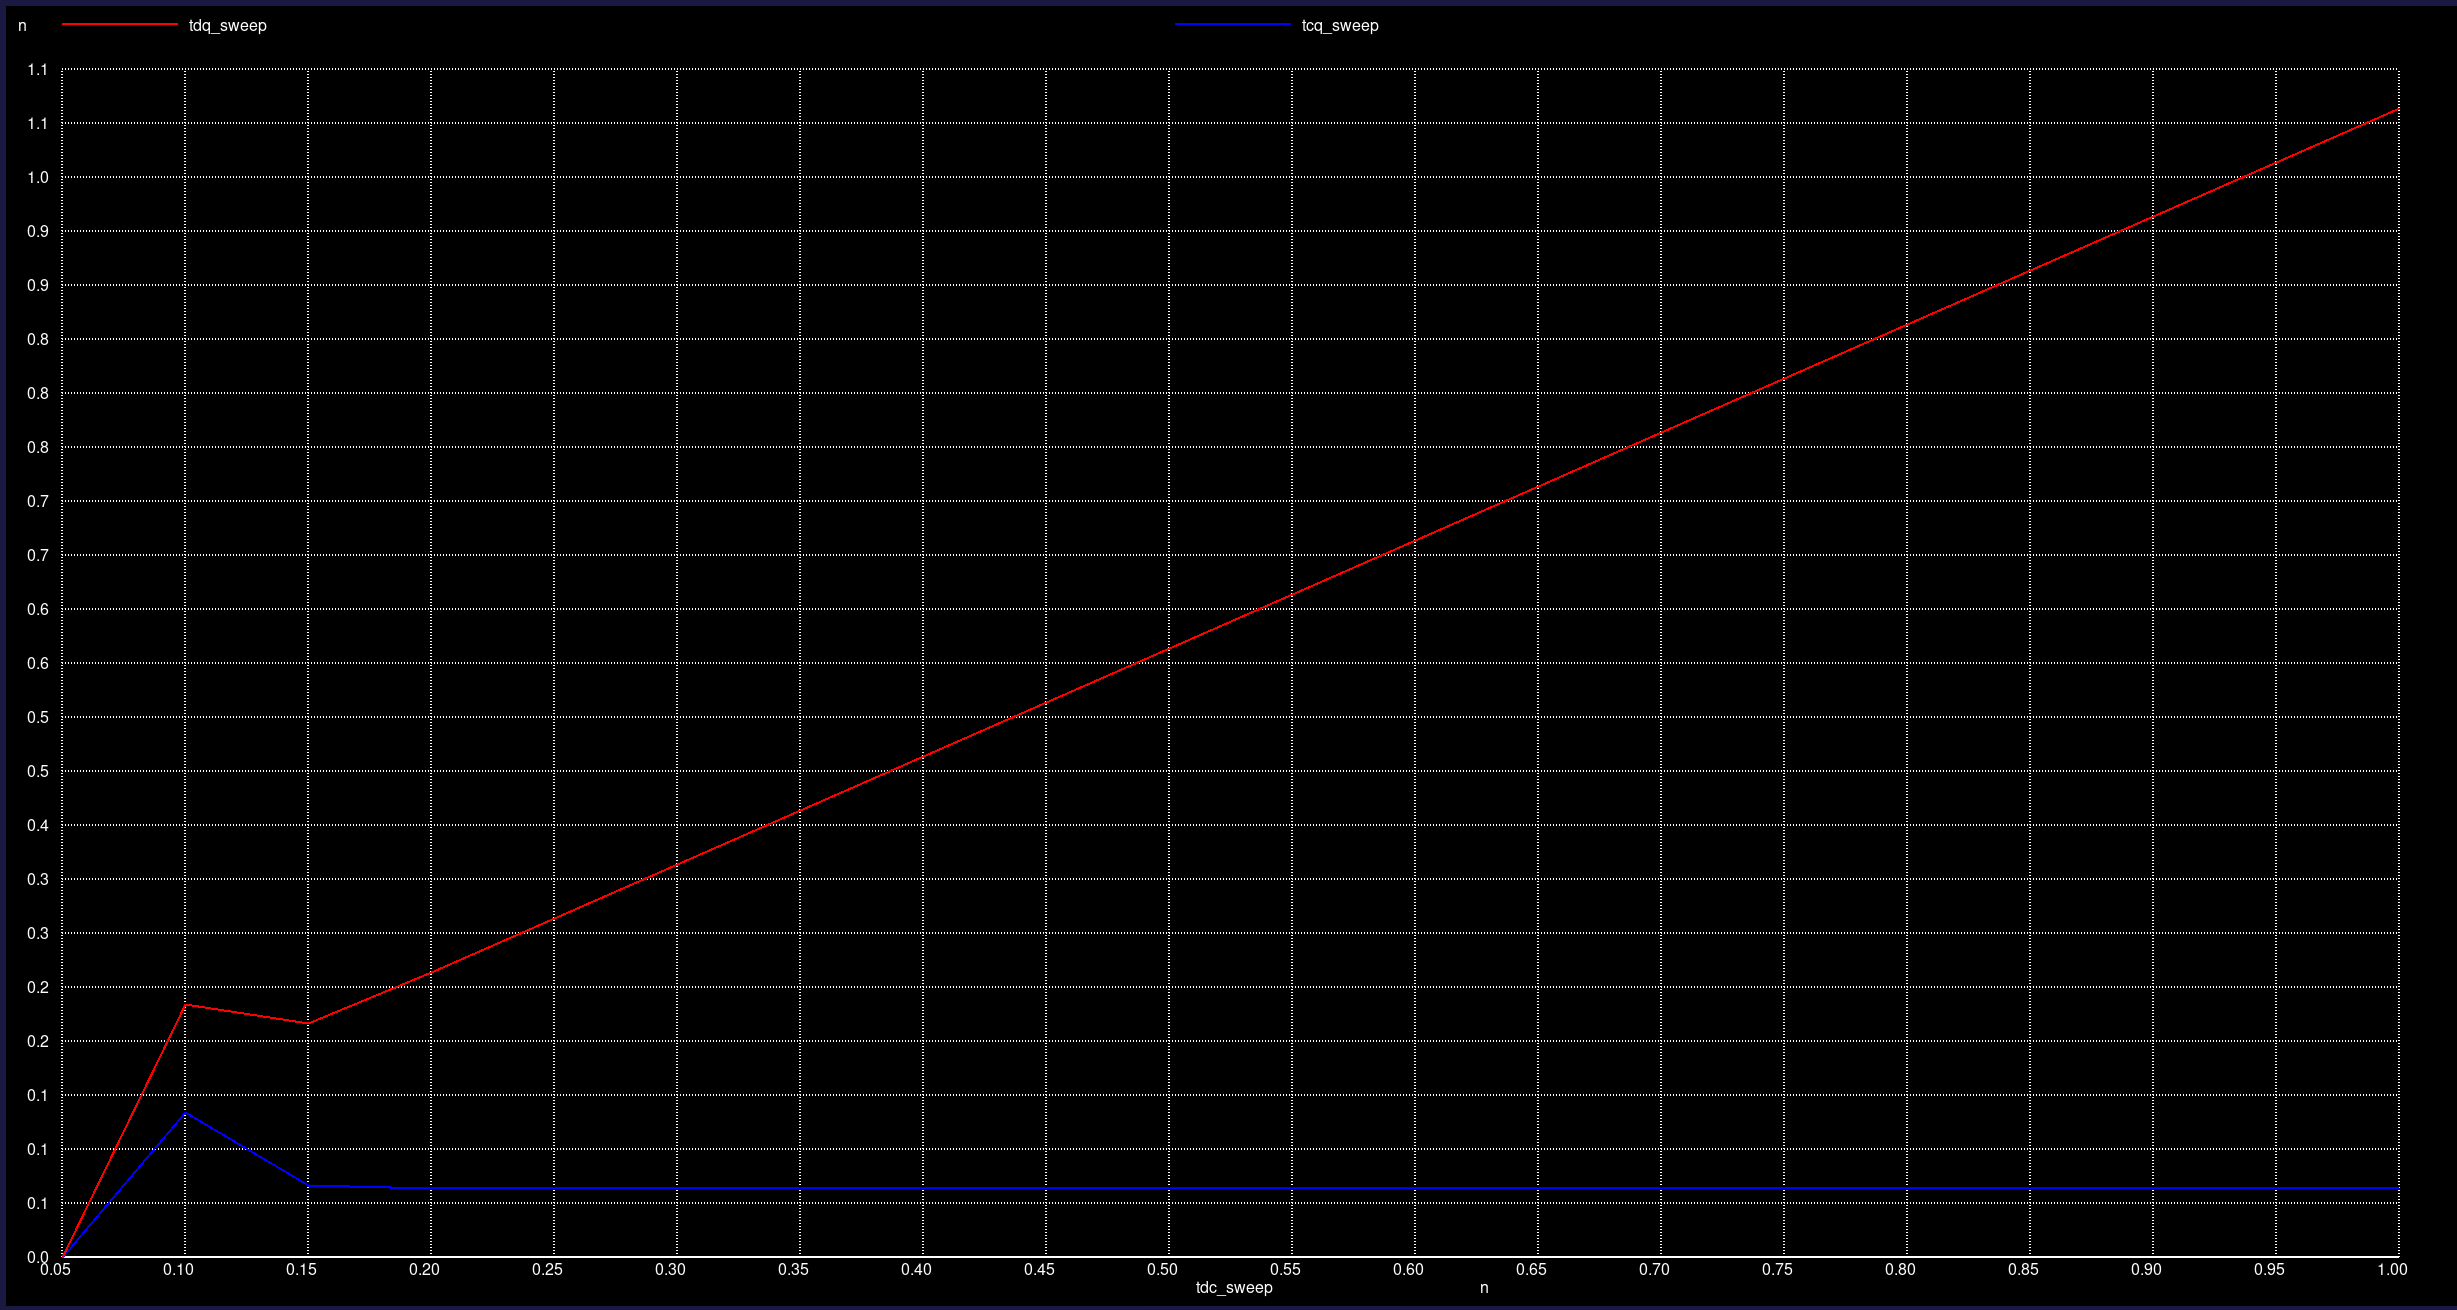
\includegraphics[width=0.85\textwidth]{figures/sweep_1a.png}

\textbf{Figure 4:} $t_{DQ}$ (red) and $t_{CQ}$ (blue) vs.\ $t_{setup}$

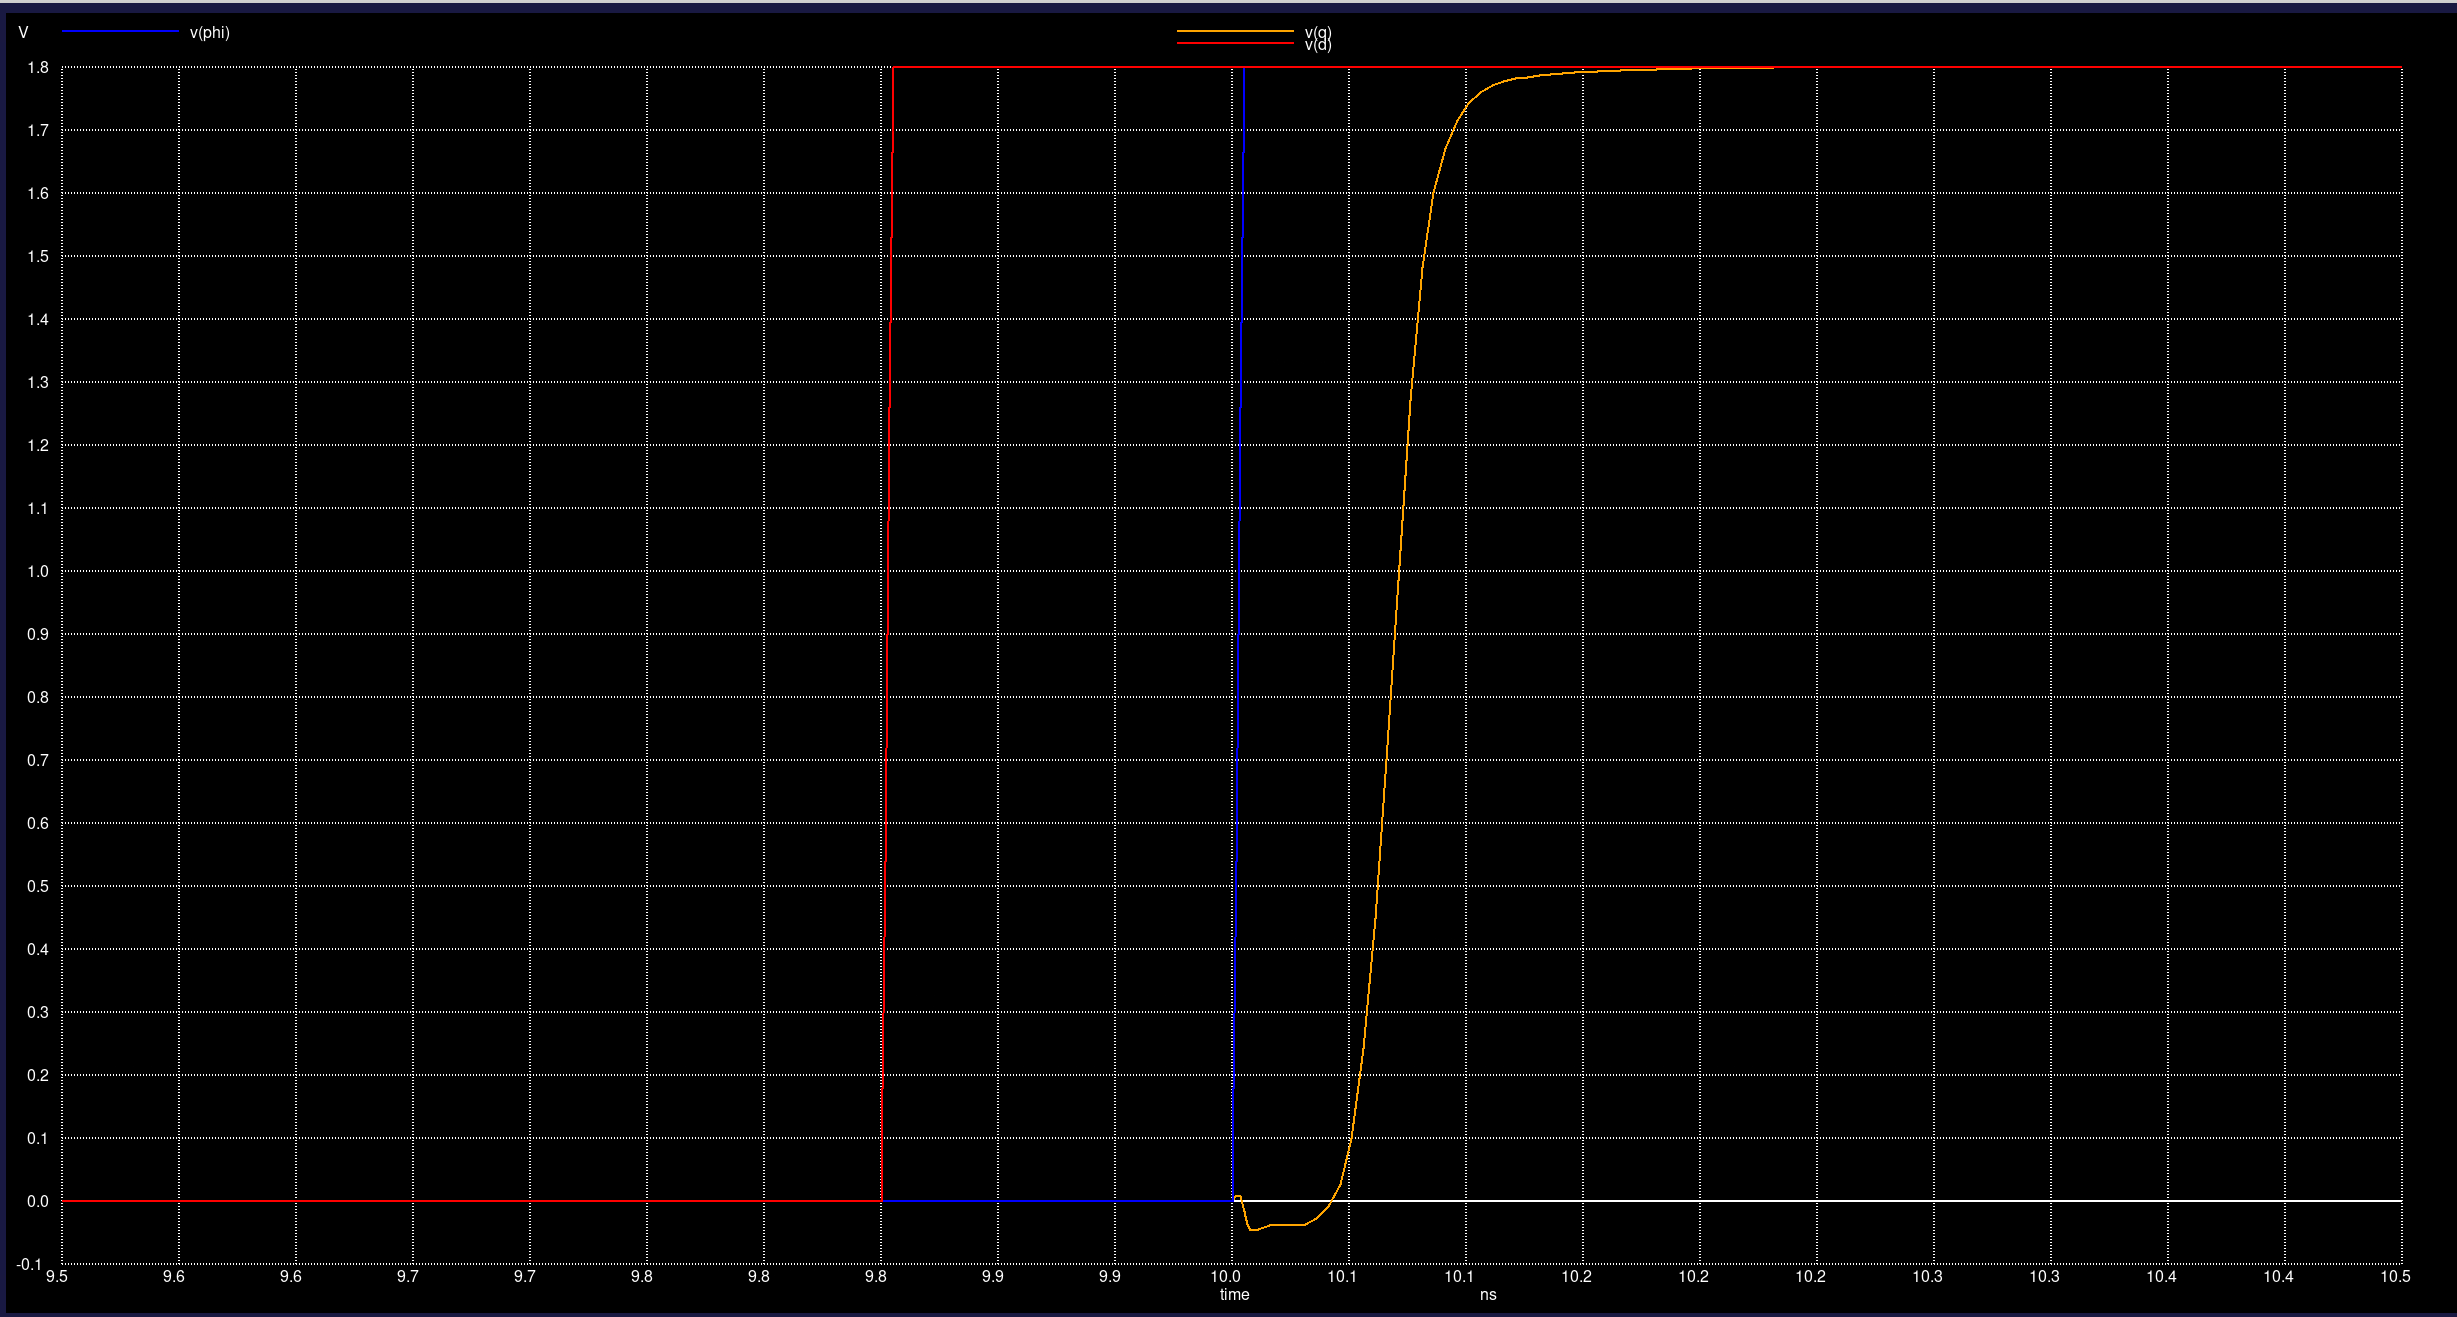
\includegraphics[width=0.85\textwidth]{figures/tran_1a.png}

\textbf{Figure 5:} $D$, $\phi$, $Q$ at the optimal setup point

\subsubsection{Calculation}

\[
\begin{aligned}
t_{setup} &= 130\ \text{ps} \\
t_{CQ} &= 80.32332\ \text{ps} \\
t_{DQ} &= t_{setup} + t_{CQ} = 130 + 80.32332 = 210.3233\ \text{ps}
\end{aligned}
\]

%%------------------------------------------------------------------------------
\section{Problem 1(b): falling edge}

\subsubsection{Schematic}

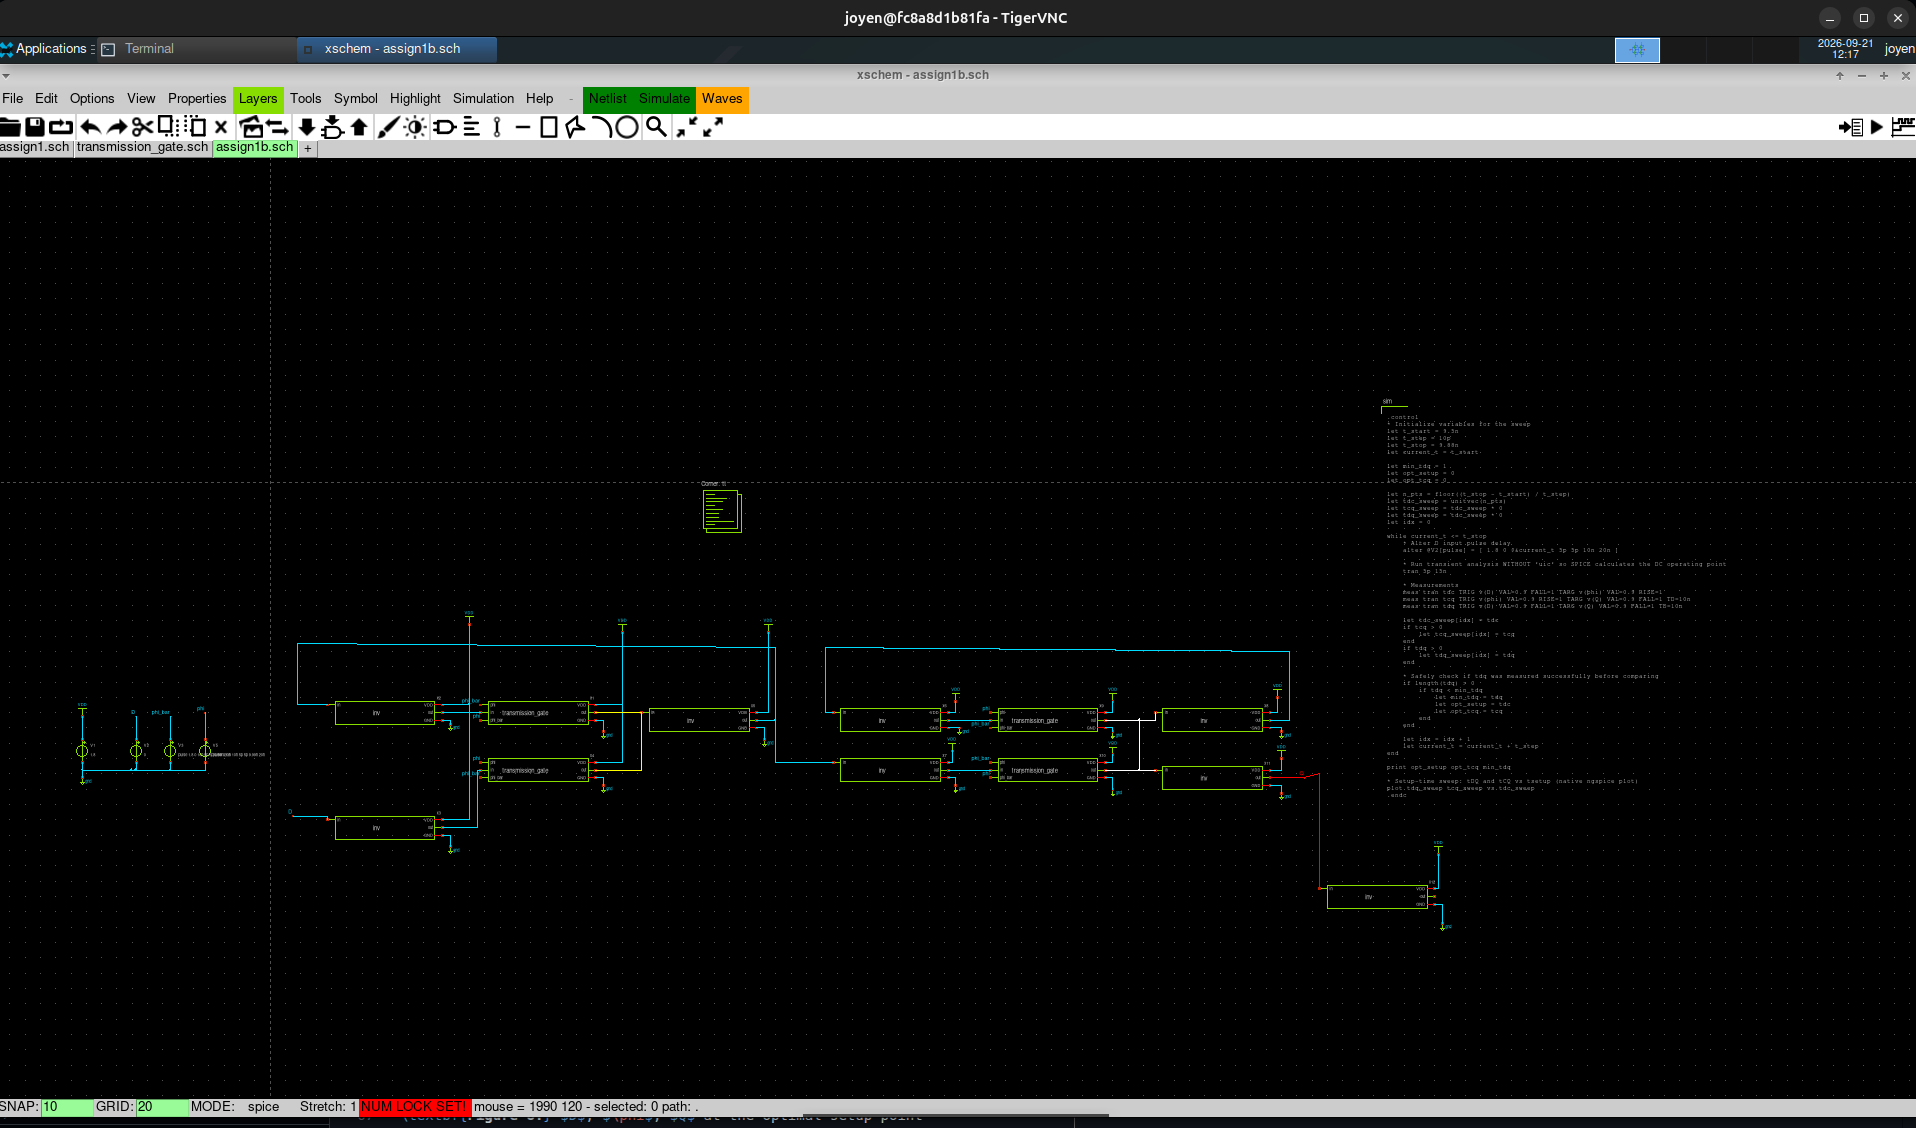
\includegraphics[width=0.95\textwidth]{figures/assign1b_schem.png}

\textbf{Figure 6:} \texttt{assign1b.sch} -- same testbench, $D$ polarity
inverted

\subsubsection{Measurement}

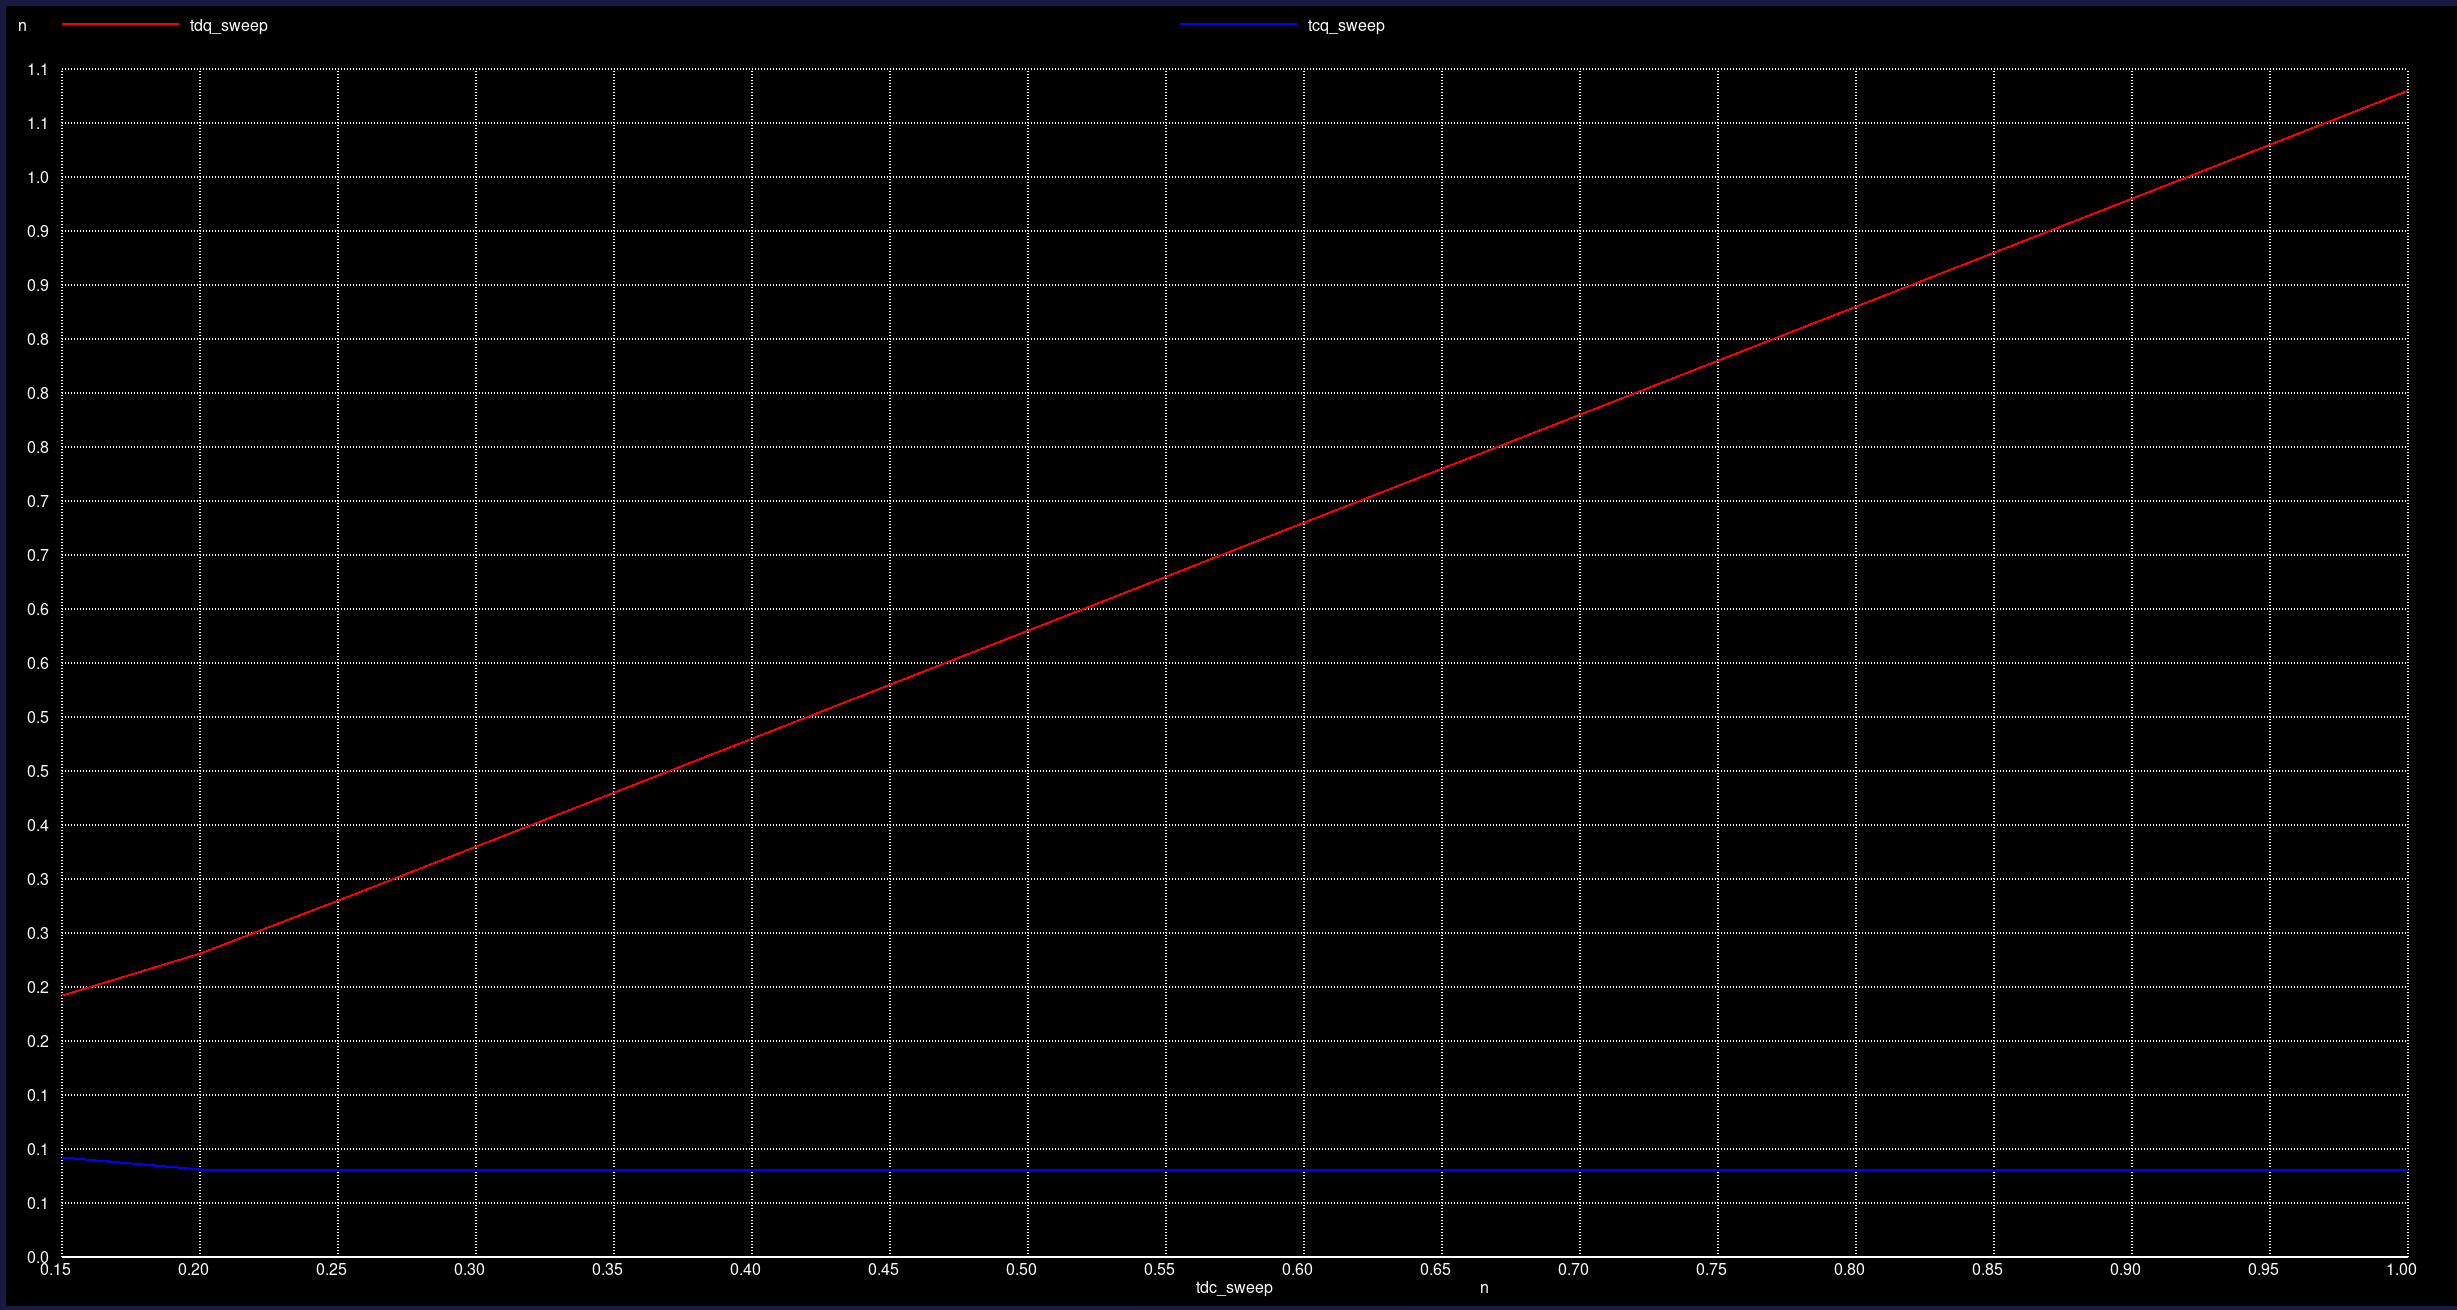
\includegraphics[width=0.85\textwidth]{figures/sweep_1b.png}

\textbf{Figure 7:} $t_{DQ}$ (red) and $t_{CQ}$ (blue) vs.\ $t_{setup}$

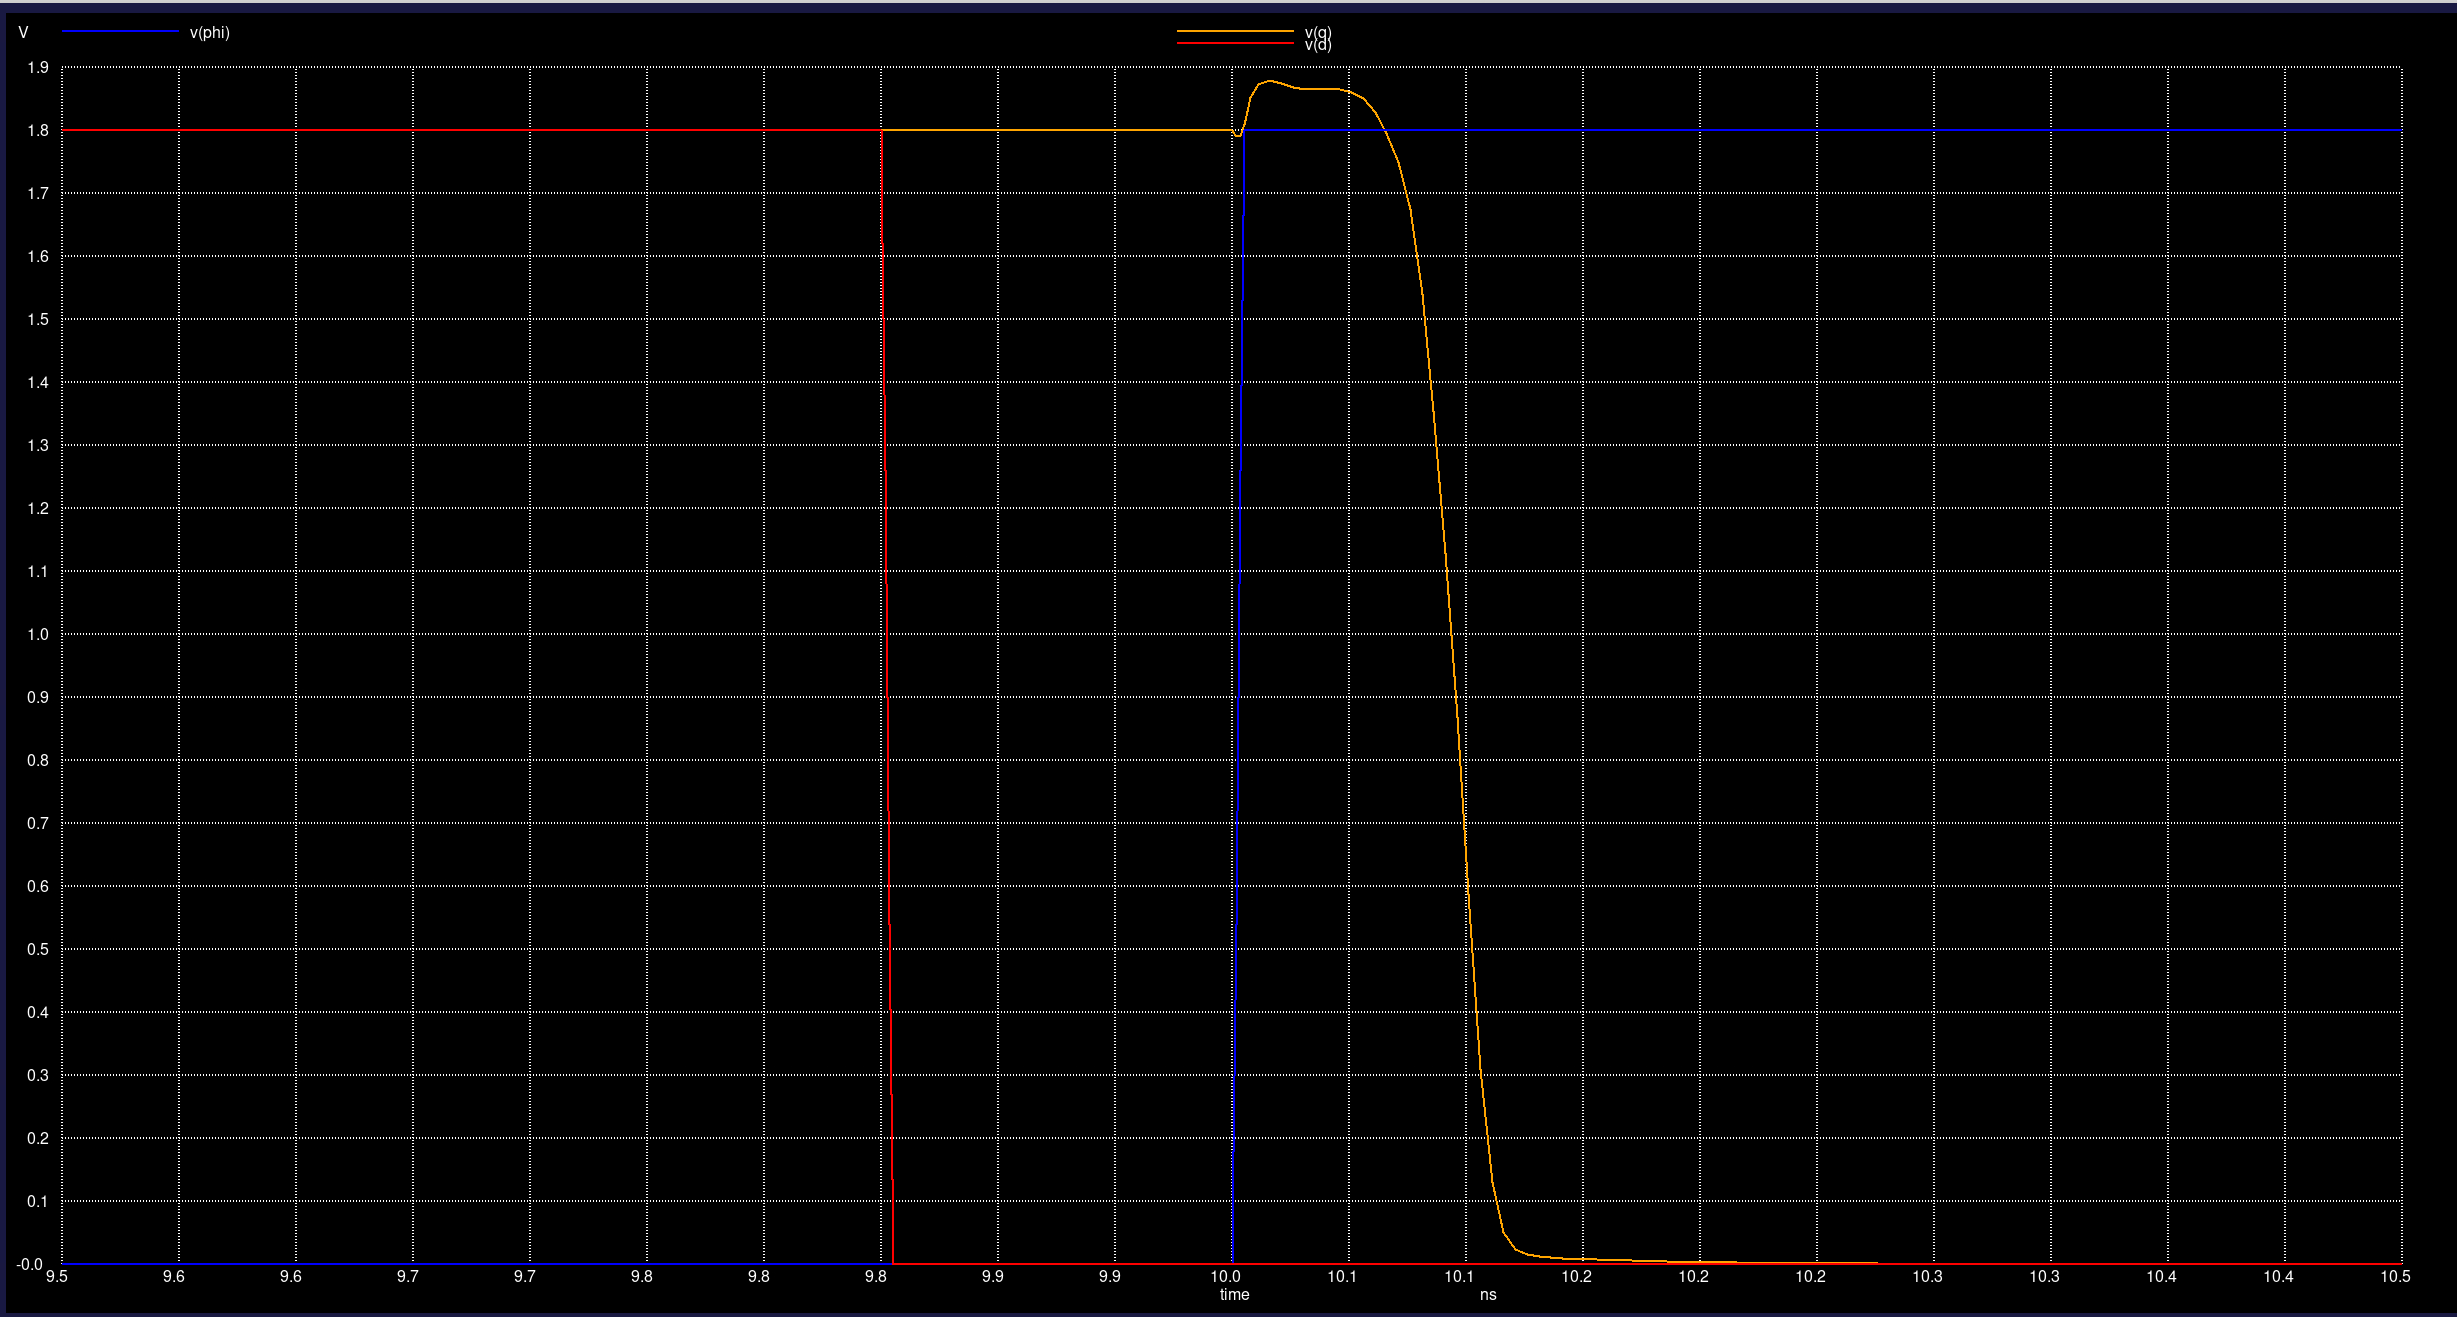
\includegraphics[width=0.85\textwidth]{figures/tran_1b.png}

\textbf{Figure 8:} $D$, $\phi$, $Q$ at the optimal setup point

\subsubsection{Calculation}

\[
\begin{aligned}
t_{setup} &= 140\ \text{ps} \\
t_{CQ} &= 100.7321\ \text{ps} \\
t_{DQ} &= t_{setup} + t_{CQ} = 140 + 100.7321 = 240.7321\ \text{ps}
\end{aligned}
\]

%%------------------------------------------------------------------------------
\section{Summary}

\begin{center}
\begin{tabular}{lccc}
\hline
 & $t_{setup}$ & $t_{CQ}$ & $t_{DQ,min}$ \\
\hline
1(a), $D/Q$ rising  & 120~ps & 93.92~ps & 213.921~ps \\
1(b), $D/Q$ falling & 140~ps & 100.732~ps & 240.732~ps \\
\hline
\end{tabular}
\end{center}
